% !TEX TS-program = xelatex
\documentclass[11pt,twoside]{report}

%---------------------------------------------------------------------------
% Packages
%---------------------------------------------------------------------------
\usepackage[margin=2.5cm]{geometry}
\usepackage[utf8]{inputenc}
\usepackage{setspace}
\usepackage{enumitem}
\usepackage{fontspec} % XeLaTeX/LuaLaTeX
% Set the global monospaced family used by \ttfamily
\setmonofont{GoMono Nerd Font Mono}[
  Scale=MatchLowercase
]
\usepackage{lmodern}
\usepackage[T1]{fontenc}
\usepackage{tabularx}
% \usepackage[utf8]{inputenc}
\usepackage{graphicx}
\graphicspath{{assets/}}
\usepackage{listings}
\usepackage{subcaption}
\usepackage{booktabs}
\usepackage{longtable}
\usepackage{float}
\usepackage{caption}
\usepackage{amsmath,amssymb}
\usepackage{hyperref}
\usepackage[numbers,sort&compress]{natbib}
\usepackage{tocloft}
\usepackage{fancyhdr}
\setlength{\headheight}{14pt}
\usepackage{listings}
\usepackage{xcolor}
\usepackage{natbib}
\usepackage{tikz}
\usetikzlibrary{shapes,arrows.meta,positioning,fit}
\captionsetup[table]{font=footnotesize, labelfont=footnotesize, justification=centering}
\captionsetup[figure]{font=footnotesize, labelfont=footnotesize, justification=centering}
\usepackage[nameinlink,noabbrev]{cleveref} % smarter refs
% Make cleveref know about listings:
\crefname{listing}{Listing}{Listings}
\Crefname{listing}{Listing}{Listings}

% Optional: include a “List of Listings” after the ToC
% \lstlistoflistings % (place in front matter where you want it)

%---------------------------------------------------------------------------
% Graphics and Listings Setup
%---------------------------------------------------------------------------
\captionsetup{font=small,labelfont=bf}
\lstset{
  basicstyle=\ttfamily\footnotesize, % now uses GoMono Nerd Font Mono
  numbers=left,
  numberstyle=\tiny,
  frame=single,
  breaklines=true,
  keywordstyle=\color{blue},
  commentstyle=\color{gray!70},
  stringstyle=\color{teal!70!black},
}
%---------------------------------------------------------------------------
% Header and Footer
%---------------------------------------------------------------------------
\pagestyle{fancy}
\fancyhf{}
\fancyhead[LE,RO]{\thepage}
\fancyhead[RE]{\nouppercase{\leftmark}}
\fancyhead[LO]{\nouppercase{\rightmark}}
\renewcommand{\headrulewidth}{0.4pt}

%---------------------------------------------------------------------------
% Spacing
%---------------------------------------------------------------------------
\onehalfspacing

%---------------------------------------------------------------------------
% Document
%---------------------------------------------------------------------------
\begin{document}

%-------------------- Front Matter --------------------
\begin{titlepage}
	\centering
	{\Huge\bfseries Title of the Thesis\\[1em]}
	{\Large Subtitle if needed\\[4em]}
	{\Large Jack Jibb\\[2em]}
	{\large School of Computing and Mathematical Sciences, University at Greenwich\\[1em]}
	{\large 2024-2025\\[4em]}
\end{titlepage}

% Abstract
\begin{abstract}
	\addcontentsline{toc}{chapter}{Abstract}
	Training quality depends not only on an athlete’s physiology but also on the road environment: long, uninterrupted climbs or low‑traffic corridors enable sustained efforts, whereas junctions, stops and heavy traffic fragment work and reduce effectiveness. This thesis investigates whether the “training suitability” of roads can be quantified and used to help cyclists plan better sessions.
	I present an end‑to‑end framework that transforms raw GPS (GPX) traces into a database of road segments annotated for training suitability. The pipeline (i) cleans and map‑matches traces to OpenStreetMap using OSRM \citep{Luxen2011}, (ii) enriches the matched geometry with road metadata (e.g., highway class, speed limit, junction density), and (iii) performs adaptive segmentation using curvature and speed‑variance cues with topology‑aware guards. Each segment is then described by spatial–temporal features and scored with a Training Suitability Score (TSS) derived from road context and observed ride dynamics. The score favours long, low‑interruption, consistent‑grade sections suited to threshold or aerobic work, and penalises frequent stops, sharp curvature, or dense junctions.
	The system supports batch ingestion of user files, segment de‑duplication and matching against an existing segment set, and a minimal web application to browse routes, visualise segments, and collect feedback. Together, these components demonstrate a practical route‑planning aid that prioritises the quality of training stimulus, not just performance ranking.
\end{abstract}

% Table of Contents, List of Figures, List of Tables
\hypersetup{pageanchor=false}
\pagenumbering{roman}

\tableofcontents
\listoffigures
\listoftables

\clearpage
\hypersetup{pageanchor=true}
\pagenumbering{arabic}

%-------------------- Main Chapters --------------------

\chapter{Introduction}
\label{chap:introduction}
High‑quality cycling training depends on being able to execute the intended effort without interruption. Professional riders often train on long climbs and low‑traffic roads chosen for this purpose; most amateurs, by contrast, plan routes with general‑purpose mapping tools and only discover mid‑ride that junctions, blind corners or traffic furniture force repeated stops and surges. The result is fragmented work and reduced training effectiveness.
This dissertation addresses that gap. I investigate whether the suitability of a road for structured training can be quantified from ride data and open mapping sources so that routes can be planned around segments that support sustained efforts. I refer to this property as \emph{training suitability}.
The proposed system ingests raw GPX traces, performs map‑matching against OpenStreetMap using OSRM, enriches the resulting paths with road metadata (e.g., highway class, speed limits and junction density), and then applies an adaptive segmentation procedure. Segments are identified using curvature and speed‑variance cues with topology‑aware guards to avoid splitting at spurious points. Each segment is described by spatial and temporal features and given a Training Suitability Score (TSS) that favours long, low‑interruption, consistent‑grade sections and penalises frequent stops or sharp bends.
On top of this pipeline, I implement (i) batch processing for large GPX collections, (ii) segment de‑duplication and matching so new routes can be expressed as sequences of known segments, and (iii) a minimal web application for exploring routes, visualising segment scores and gathering feedback.
In summary, this work aims to move route planning beyond performance rankings towards the deliberate selection of roads that maximise training stimulus. The remainder of this chapter provides background and states the research objectives that guide the study.
\section{Background}


\section{Research Objectives}
\label{sec:research-objectives}
This dissertation investigates whether the \emph{training suitability} of roads can be quantified from ride data and open map sources to support route planning for structured efforts. The objectives are:

\begin{enumerate}[label=O\arabic*., leftmargin=2.2em]
	\item \textbf{Define ``training suitability''.} Formalise a segment-level construct that captures the ability to execute sustained work with minimal interruptions and predictable load.
	\item \textbf{Build a reproducible map-matching pipeline.} Establish a deterministic GPX~$\rightarrow$ OSM route pipeline (OSRM \citep{Luxen2011}) with monotonic streaming matching and topology-aware guard windows for leg boundaries.
	\item \textbf{Develop segmentation methods.} Compare candidates for route segmentation:
	      \begin{enumerate}[label=O3\alph*., leftmargin=2.5em]
		      \item curvature/heading and grade change-points,
		      \item speed-variance and stop-density cues,
		      \item multi-scale (wavelet \citep{Sharifzadeh2005}) change detection,
		      \item topology-aware guards (junction density, crossings),
		      \item greedy vs.\ dynamic-programming formulations.
	      \end{enumerate}
	\item \textbf{Engineer segment features.} Design a feature schema: length, elevation gain, mean/variance of grade, curvature, stop/junction density, speed-limit, highway class, surface/cycleway tags, and simple traffic proxies derived from OSM metadata.
	\item \textbf{Specify a TSS model.} Create (i) a transparent rule-based baseline and (ii) a learned model (e.g., logistic/ordinal regression or learning-to-rank) mapping features to a scalar training suitability score.
	\item \textbf{Ground-truth construction.} Derive labels from ride dynamics (e.g., proportion of time in target zone, pause frequency, % of clean power without surges) and small expert annotations; construct pairwise preferences for ranking.
	\item \textbf{Validate alignment with training intent.} Test whether TSS correlates with: (a) sustained power feasibility, (b) low interruption frequency, (c) subjective suitability ratings.
	\item \textbf{Ablation and robustness.} Quantify sensitivity to GPS noise, map-matching errors, missing OSM tags, and urban vs.\ rural context; evaluate cross-region generalisation.
	\item \textbf{Efficiency.} Measure throughput (GPX points/s) and memory footprint for streaming vs.\ batch; target near real-time feedback for typical rides.
	\item \textbf{Segment library operations.} Deduplicate, index, and match new routes to an evolving segment set; assess match precision/recall and update policies.
	\item \textbf{Human-in-the-loop feedback.} Prototype lightweight feedback (thumbs-up/down or pairwise choices) and test whether incorporating it improves ranking metrics.
	\item \textbf{Reproducibility and privacy.} Ensure runs are reproducible (configs, seeds, versions) and only aggregated, per-segment stats persist (no user-identifiable ride data).
\end{enumerate}

\subsection{Research Questions and Hypotheses}
\begin{description}[leftmargin=2.2em, style=nextline]
	\item[RQ1:] Which segmentation criterion best aligns with actual changes in riding regime?
	\item[H1:] Multi-cue segmentation (curvature + stop density + grade) yields higher boundary F1 vs.\ single-cue methods.

	\item[RQ2:] Can a learned TSS outperform a rule-based baseline in ranking segments for sustained efforts?
	\item[H2:] A learning-to-rank model (using the feature schema) achieves higher NDCG@k and Kendall’s $\tau$ against expert/pairwise labels.

	\item[RQ3:] Do topology-aware guard windows reduce spurious splits near complex junctions?
	\item[H3:] Guarded segmentation reduces over-segmentation rate and improves segment continuity (median segment length, lower split-at-junction rate).

	\item[RQ4:] Does TSS correlate with feasibility of holding target power/HR on held-out rides?
	\item[H4:] Segment-level TSS shows significant positive correlation (Spearman $\rho$) with \% time-in-zone and low pause/surge counts.

	\item[RQ5:] How robust is the pipeline to GPS noise and incomplete OSM tags?
	\item[H5:] Performance degrades gracefully under noise injection (≤10\% drop in NDCG@10 at realistic jitter) and missing-tag ablations.

	\item[RQ6:] Can the segment library generalise across regions?
	\item[H6:] Models trained in Region~A retain ranking performance within 5–10\% NDCG on Region~B after simple reweighting or calibration.
\end{description}

\subsection{Planned Evaluation (Datasets \& Metrics)}
\begin{itemize}[leftmargin=2.2em]
	\item \textbf{Data:} Your GPX set (post map-matching); optional power/HR to derive time-in-zone; small expert labels or rider pairwise preferences.
	\item \textbf{Segmentation metrics:} Boundary precision/recall/F1 against regime-change heuristics; segment continuity (median length, split-at-junction rate).
	\item \textbf{Suitability metrics:} Spearman $\rho$ with feasibility proxies; AUC/accuracy for suitable vs.\ unsuitable; ranking NDCG@k / MAP; calibration (ECE).
	\item \textbf{Robustness:} Noise sweeps (GPS jitter), missing-tag ablations, cross-region transfer; report deltas on main metrics.
	\item \textbf{Efficiency:} Throughput (pts/s), end-to-end latency per ride, memory peak.
	\item \textbf{Ablations:} Feature-group and cue ablations (remove curvature, remove stops, remove grade) to quantify contribution.
\end{itemize}

\chapter{Literature Review}
\label{chap:litreview}

\section{Training Suitability and Segmentation Algorithm Design and Analysis}

\subsection{Research Objectives}
The purpose of creating an algorithmic approach to categorizing and segmenting a GPX route is to be able to rapidly and systematically construct new routes based on the requirements of the rider's training plan.
It makes sense intuitively to segment a route, so riders does not have to analyse every part of a map to determine where to send their route. Riders are specifically interested in sections of the route such as climbs, descents, busy roads, and gravel.
The objective of research should be to come up with a suitable method of segmentation, and subsequent categorization of the resulting segments so riders can select ones that suit their training needs.
\\
Intuitively, we can segment a route by the roads that it follows, when a route changes roads, we add a segment. However this can prove more difficult to formalize, as
a road can have many intersections. How can we categorize a segment by road name but also have node values that connect to other road names that may or may not be part of the same segment?
The following research applies to the problem of Segmentation, and how we may approach defining a route segment formally.

\subsection{Algorithmic Approaches to Segmentation and Categorization}
\subsection{Methodological Considerations and Assumptions}
Firstly we must obtain a GPX file. This is give from either a new or existing activity. It can be downloaded in many ways, either from common fitness websites (Strava, Garmin, MapMyRide, etc.), or directly
downloaded from a GPS device. Either way, there are some standards we can take advantage of. Each GPX is an XML-style file. Here is a snipped from
a GPX file used in testing the system:
\begin{verbatim}
<trk>
  <trkseg>
    <trkpt lat="38.82032" lon="-104.861694">
      <time>2024-08-06T13:12:58.000Z</time>
      <ele>1884.8</ele>
      <extensions>
        <power>168</power>
        <tpx1:TrackPointExtension>
          <tpx1:atemp>20</tpx1:atemp>
          <tpx1:hr>123</tpx1:hr>
          <tpx1:cad>65</tpx1:cad>
        </tpx1:TrackPointExtension>
      </extensions>
    </trkpt>
    ...
  </trkseg>
</trk>

\end{verbatim}
It's clear to see that it is a hierarchical tree structure, with various metadata. Not all of the data is named constantly, so it is important
to consider variations in naming. This can be normalized along with any other normalization processes.
\\
Once downloaded, they must be normalized and processed. This can be done by converting to a standardized JSON structure, where each object contains at least Latitude, Longitude, Elevation, and timing data.
After this, some processing should be done to remove any erroneous values. Simply detecting 0s or NaN values in the data stream is sufficient, and the missing data can be interpolated with the average of the surrounding present values.
Next, derived metadata, such as speed or heading, should be calculated mathematically using the Haversine formula and trigonometry, and added as an additional extension in the JSON file.

\subsection{Pulling Map Data}
A useful library for python called OSMnx exists, which allows easy and efficient pulling of API data from the OpenStreetMap database. This is what we will use to correct the GPS data, and to enrich the data for segmentation and categorization.
To do this, we use the \texttt{os.graph\_from\_bbox()} function to pull only nearby data (within the bounding box of the route). The approach is as follows:
\begin{enumerate}
	\item Find the largest and smallest coordinates in the route
	\item Generate a bounding box of the extreme coordinates
	\item Send the bounding box to a function that pulls the data from OSM
\end{enumerate}


\section{Training Suitability Scoring}

\subsection{Research Objectives}
\subsubsection{Construct and Scale Definition}
\begin{enumerate}
	\item \textbf{Define the construct}: Precisely define what TSS measures (segment suitability for endurance, tempo/threshold, VO$_2$max, anaerobic/neuromuscular work).
	\item \textbf{Score scale and calibration}: Design a bounded scale (e.g., 0--100) with interpretable anchors; ensure monotonicity with increasing segment challenge.
	\item \textbf{Task taxonomy}: Map segments to training intents; specify how a single segment can be suitable for multiple intents with different scores.
\end{enumerate}

\subsubsection{Data and Feature Engineering}
\begin{enumerate}
	\item \textbf{Core geometry features}: Length, elevation gain/loss, grade distribution (percent time in grade bins), curvature/turn density, stop density, junction density.
	\item \textbf{Dynamics features}: Speed variance, acceleration peaks per km, cadence/power variability (if available).
	\item \textbf{Context features}: Surface type, traffic class (if derivable), wind exposure (proxy via openness), time-of-day/week effects (optional).
	\item \textbf{Directionality}: Treat opposing directions as distinct; verify feature asymmetry (e.g., climb vs. descent).
	\item \textbf{Sensor fallbacks}: Specify safety fallbacks when power/HR are absent (e.g., speed–grade model, elevation-derived effort proxies).
\end{enumerate}

\subsubsection{Personalisation vs. Population Baseline}
\begin{enumerate}
	\item \textbf{Dual scoring}: Produce both (a) population TSS (sensor-agnostic) and (b) optional rider-adjusted TSS using FTP/HR zones when available.
	\item \textbf{Normalization}: Ensure comparability across riders and devices (e.g., z-scores by region/segment length, or duration-normalized metrics).
\end{enumerate}

\subsubsection{Algorithm Design}
\begin{enumerate}
	\item \textbf{Model family}: Compare transparent formula-based models (weighted feature sum with calibrated bins) vs. learned models (ordinal regression / pairwise ranking).
	\item \textbf{Weight learning}: Learn weights from coach labels or pairwise “A more suitable than B” judgments; constrain for interpretability.
	\item \textbf{Multi-objective scoring}: Support per-intent heads (Endurance/Threshold/Neuromuscular) sharing a common feature backbone.
	\item \textbf{Uncertainty}: Output a confidence/uncertainty score (e.g., via bootstrap or ensembling) for downstream UI.
\end{enumerate}

\subsubsection{Validation and Evaluation}
\begin{enumerate}
	\item \textbf{Reliability}: Test consistency on repeated rides (ICC, coefficient of variation) under GPS noise and sampling-rate changes.
	\item \textbf{Criterion validity}: Correlate TSS with expert/coach ratings and with proxy physiology (normalized power, % time in Z4–Z6, HR drift).
	\item \textbf{Discrimination}: AUC/average precision to separate segments intended for different training zones.
	\item \textbf{Calibration}: Reliability plots (expected vs. observed difficulty bins).
	\item \textbf{Generalisation}: Cross-validate across geographies (urban/rural, hilly/flat) and seasons; check domain shift.
\end{enumerate}

\subsubsection{Robustness and Edge Cases}
\begin{enumerate}
	\item \textbf{GPS/Map-matching noise}: Stress-test with perturbed trajectories; target $\leq$5\% score drift.
	\item \textbf{Segment length effects}: Ensure fairness across short vs. long segments (length-aware normalization).
	\item \textbf{Outliers}: Downweight extreme rides (e.g., device glitches, group sprints) to protect segment baselines. Can filter out data points above
	      certain standard deviation value or absolute ceiling (2000+ watts/200rpm/250hr, etc...).
\end{enumerate}

\subsubsection{Operational Objectives}
\begin{enumerate}
	\item \textbf{Versioning}: Define TSS schema \& model versioning.
	\item \textbf{Explainability}: Provide per-segment feature attributions (e.g., SHAP) for UI tooltips (“score driven by 8\% average grade and high curvature”).
	\item \textbf{Privacy}: Use only aggregated segment features for public stats; no storage of user-identifiable ride data.
\end{enumerate}

\subsubsection{Datasets and Ground Truth}
\begin{enumerate}
	\item \textbf{Label collection}: Design a small expert-annotated set (coach ratings / pairwise preferences) covering common segment archetypes.
	\item \textbf{Benchmark split}: Publish/train/val/test splits across regions and segment types; document acquisition and preprocessing.
\end{enumerate}

\subsection{Approaches to Suitability Scoring}
\paragraph{Sharifzadeh et al. "Change Detection in Time Series Data Using Wavelet \citep{Sharifzadeh2005} Footprints"}
An interesting approach to Suitability scoring relates to Fast Fourier Transforms, and a convolution approach comes from Medhi Sharifzadeh et al, from the University of Southern California, introducing a concept known as
"wavelet footprints" as a compact, multi-resolution approach to representation of spatial-temporal trajectories. Wavelet footprints are a  more granular version of the Wavelet Transform, which in turn is a version of the Fourier Transform. The approach involves using Wavelets to transform a signal into the "Wavelet Domain".
The smaller the wavelet, the more reactive it will be to change in the original signal, so by adjusting the size of the wavelet, the signal can be filtered to be more or less reactive to change.
Wavelet footprints have an advantage over the general Wavelet transform, where they only retain the most significant components. This is done by having wavelets occur in orthoganal sets.
Due to Heisenberg's Uncertainty Principle, it is impossible to perfectly describe both the frequency content of a signal and the location in time of the signal. Time-domain and Frequency-Domain analysis in this regard are
at opposite ends of the spectrum, but the Wavelet Domain sits in the middle, allowing for a sliding scale value, where a larger scale gives more frequency and less time resolution, while smaller scales give less frequency, and more time resolution.

The advantage of using wavelet footprints over the Fourier Transform means that it is possible to isolate points in the signal where significant changes occur in specific metrics, or combination of metrics, allowing flexibility in choosing
what conditions must be met to enact a segmentation.

\paragraph{Indoor Cycling Association: "How Much Time in the Red Zone?"}
This article details a breakdown of the 7-training-zone model, which provide a good template for cutoff times for tuning Wavelet Footprints for analysing the GPX signal.
The general consensus is having 5 zones is a good compromise between continuous training definitions (specific power numbers) and binary (hard or easy). While the article describes 7 zones,
Zones 1-3 all fall outside of the hour range, which for the purpose of segment analysis would be fairly useless. The 5-Zone model approach
has good suitability to wavelet analysis, since small scale values for a wavelet would detect short burst efforts, while larger scales will detect longer, sustained effort.
Having 5 zones allows for a reduced scale array, contributing to higher performance. \ref{fig:7zone}, courtesy of the Indoor Cycling Association, breaks down each zone. Zones 3-7 will be used for Wavelet Analysis.
\begin{figure}[htbp!]
	\begin{center}
		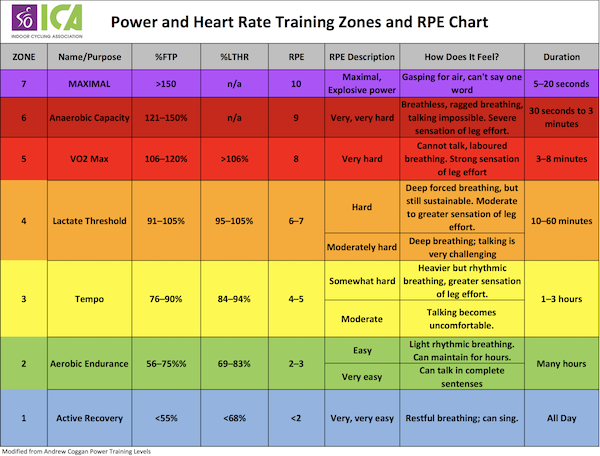
\includegraphics[width=0.6\textwidth]{zones.png}
	\end{center}
	\caption{The 7 Zone Training Model, courtesy of Indoor Cycling Association}
	\label{fig:7zone}
\end{figure}

\paragraph{Sean Hurley: "Normalized Power \citep{Hurley2020}: What It Is and How to Use It"}
TrainerRoad writer Sean Hurley provides a useful and consise definition of Normalized Power (NP), a metric invented by Dr. Andrew Coggan in his book \textit{Training and Racing With a Power Meter}. NP
"reflects the disproportionate metabolic cost of riding at high intensity, by weighting hard efforts and deemphasizing periods of easy spinning", according to Dr Coggan.
Essentially, NP approximates what power a rider could have put out for the same effort, if their effort was steady-state. While it is not a completely accurate metric for effort, it is a really
good indication of power variability, and as such is useful in determining the type of effort of a segment. The algorithm for determining NP is as follows:
\begin{enumerate}
	\item Calculate a rolling 30 second average power for the duration
	\item Raise each rolling average value to the fourth power.
	\item Determine the average of all the rolling values
	\item Take the fourth root.
\end{enumerate}
For an input power signal, $P(t)$ over interval $(0,N)$, the formula for Normalized Power (NP) is:
\[
	\mathrm{NP} = \bigg( \frac{1}{N} \sum_{i=1}^{N}\big(\overline{P}_{r}(i)\big)^{4}\bigg)^{1/4}
\]
where $P_r$ is the 30 second rolling average power starting at point i in the power data array.
\subsection{Methodological Considerations and Assumptions}
In order to classify a segment, it is necessary to know what an athlete values in training. As a cyclist, I have used my own experience to compile this list:

\begin{itemize}
	\item Type: What is the categorization of the road? (A, B, Service, Motorway, Bike path)
	\item Surface: What is the surface of the road made of? (Tarmac, concrete, gravel, dirt, wood?)
	\item Behaviour: How does the road act? (Straight, gradual bends, sharp curves, switchbacks)
	\item Safety: How safe is this route? Are there a lot of accidents, is there a lot of commercial traffic?
	\item Elevation: Is this route a consistent gradient, is it flat, uphill, downhill, rolling?
	\item Length: How long is the route in metres.
\end{itemize}

Implementing a summative score that represents a segment will also benefit from taking rider metrics, such as Power, HR, Cadence, and Speed.
As a cyclist or group of cyclists ride a specific segment, the better picture we get of the route, as the average values will be a good representation
of the training suitability of the route.
\begin{itemize}
	\item \textbf{Power:} All cyclists have different power thresholds; in other words, two cyclists may be going the same speed up a climb, but one may be going all out, and another just going easy.
	      They may not even have the same power output. The one going easy could have a higher power output than the person going all out, depending on their weight. As such absolute power is a bad reference
	      point for training suitibility. Rather, we need to focus on power variation, as well as power curve. A power curve is the integration of all power numbers over a duration of exercise, plotted average power in watts on the y-axis,
	      and max sustained duration for that average power on the x-axis. The graph tends to look like an exponential decay function. An example of my own personal cumulative power curve in 2024 is shown in \ref{fig:jibb_powercurve}.
	      \begin{figure}[htbp!]
		      \centering
		      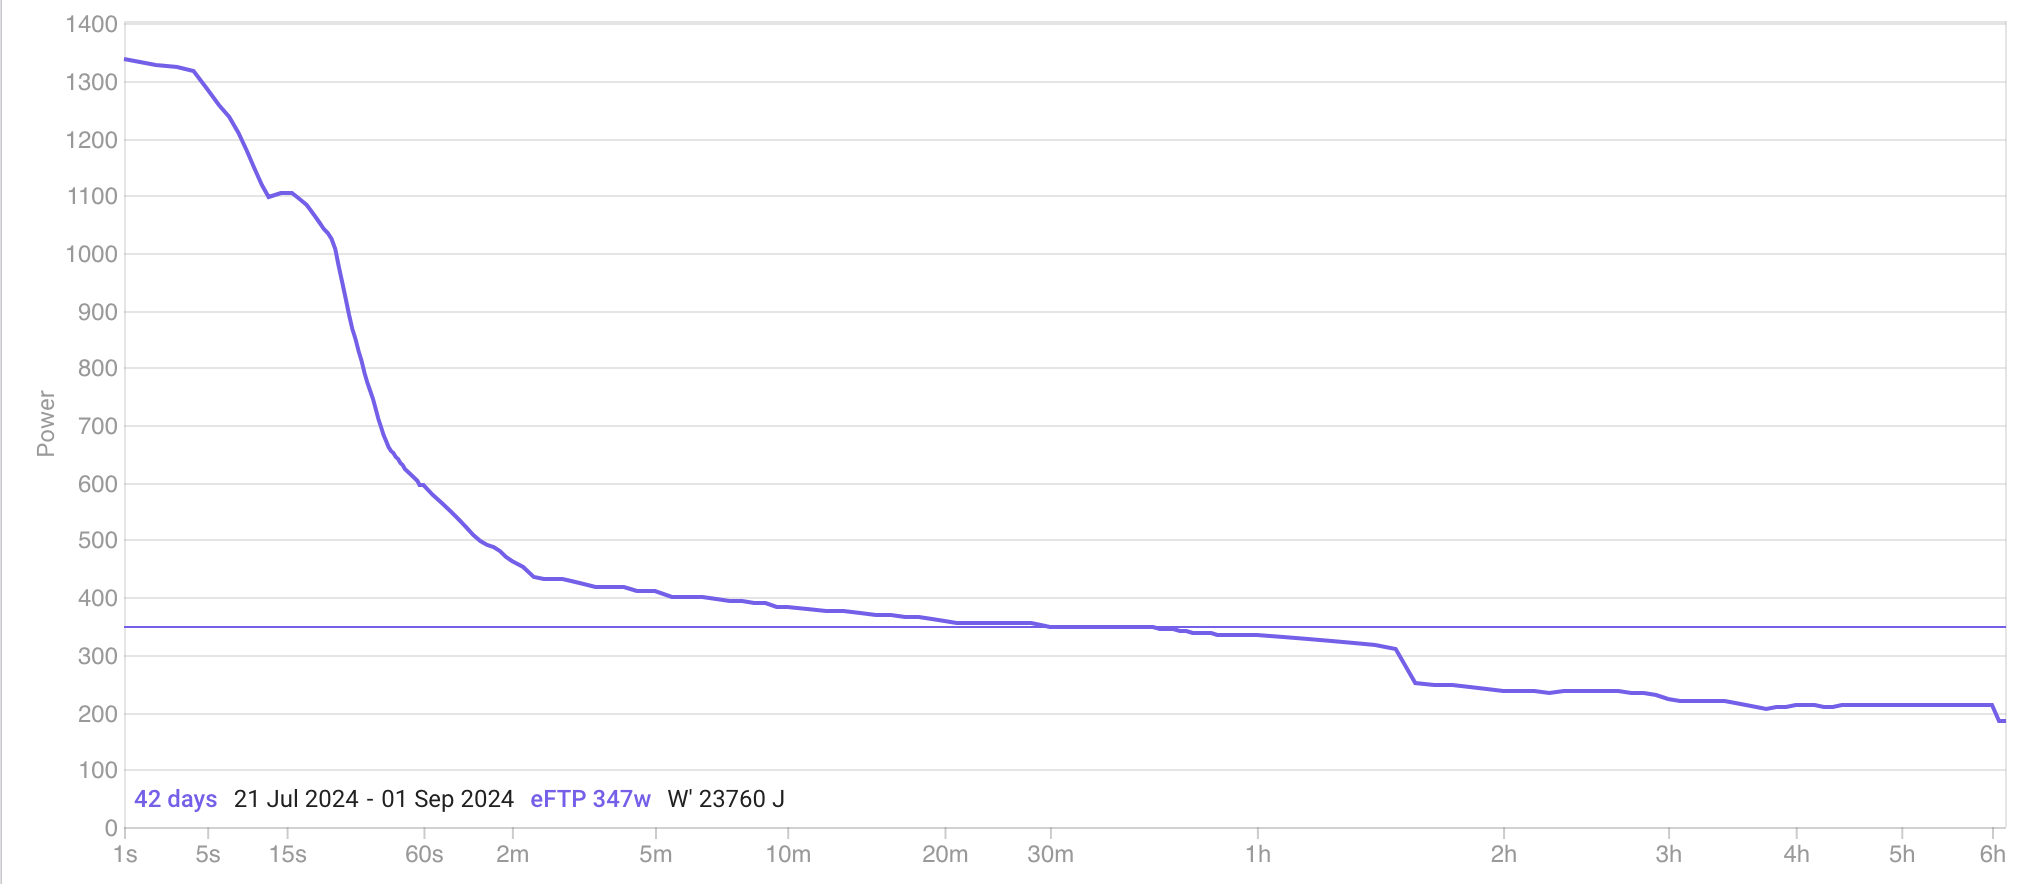
\includegraphics[width=0.8\textwidth]{jibb_powercurve.png}
		      \caption{My Power Curve for August, 2024. The power curve can estimate what would be considered "hard" for an athlete at a given duration. Image courtesy of \textbf{intervals.icu}}
		      \label{fig:jibb_powercurve}
	      \end{figure}
	\item \textbf{Route Terrain:} Hilly or technical terrain (such as lots of sharp corners or non-pavement roads) can significantly affect how good a route is for training, but
	      in different ways. Hilly terrain could be really good for consistent efforts, if the gradient is sustained, but if there are a lot of short, steep climbs, it would be harder to maintain
	      any consistency in effort. Likewise, gravel or dirt roads could be good for endurance if they are consistent, but throw in some sharp corners, and suddenly you have to brake a lot more, accelerate,
	      and even focus on balancing more, which can induce more fatigue. Terrain is probably the most important metric that is intrinsic to the route iself.
	\item \textbf{Safety:} Safety is obviously very important in general when cycling, but it also plays a big part in performance. Having to focus on keeping safe on the road often means
	      being ready or having to brake or slow down to avoid getting into dangerous situations. If a road can be considered "safe" (think long straight bike paths, or straight roads with very little traffic), then
	      the athlete is free to focus more on their effort. To consider safety is a complicated problem, since there are many aspects. One method to consider could be to come up with a points system, and apply danger points
	      as a suitibility metric. Every "unsafe" property of a road can add danger points to the segment, and a subjective scoring system could be put in place initially, and in the future, a machine learning approach could be used.
\end{itemize}

\begin{enumerate}
	\item Safety (a composite metric defined by various factors, could also be gathered collectively from rider feedback)
	\item Difference between Average and Normalized Power (in Watts/Kg)
	\item Length (of segment)
	\item Elevation Gain (or loss)
	\item Road Quality
	\item Absolute Normal Distance Change (aka how twisty the road is)
\end{enumerate}

\section{LSEPI Analysis}
\subsection{Legal}
\subsection{Social}
\subsection{Ethical}
\subsection{Political}
\label{sec:lsepi}
% LSEPI analysis content.

\chapter{Requirements}
\label{chap:requirements}
\section{Software Requirements Specification (SRS)}
\label{sec:srs}
% ISO/IEC/IEEE 29148 \citep{ISO29148}-compliant structure
\subsection{Purpose and Scope}
\label{sec:purpose}
The purpose of this Software Requirements Specification is to define the functional and non-functional requirements
for the GPX-Based Route Segmentation and Analysis System. This system enables end users (primarily cyclists and coaches)
to upload recorded GPX ride data or draw routes on a web map, automatically segment the route into reusable “segments,”
match them against a central database of known segments, and compute training-relevant statistics (Training Suitability Score, TSS).
The SRS covers requirements for both \emph{upload mode} (GPX ingestion, segmentation, database updates) and \emph{query mode}
(route matching without creation).

\subsection{Intended Audience and Reading Suggestions}
\begin{itemize}
	\item \textbf{Developers:} Read entire SRS to understand system scope, functional interfaces, and data models.
	\item \textbf{Testers:} Focus on Section \ref{sec:specific} (Specific Requirements) for test case derivation.
	\item \textbf{Stakeholders (coaches, cyclists):} Sections \ref{sec:purpose}–\ref{sec:overview} provide high-level understanding of capabilities.
\end{itemize}
\subsection{Overall Description}
\label{sec:overview}
\subsubsection{Product Perspective}
This system is a standalone web service that is built on a LAMP-like technology stack (Linux, Nginx, MySQL, Flask), augmented by Python and Dockerized C++ processing engines.
It integrates with third party mapping libraries (OpenStreetMap, Overpass, Osmium and OSRM). Conceptually, it acts as a data processor, taking user's GPX files from their GPS-enabled devices,
and processing them against a central database. The system acts as an ETL (Extract-transform-load) pipeline for incoming GPX files, as well as a query engine
for user-inputted drawn map routes from a map drawing system.

\subsubsection{Product Functions}
\begin{itemize}
	\item \textbf{GPX Ingestion:} Accepts GPX 1.1 uploads, applies privacy-filter trimming, and parses into coordinate streams.
	\item \textbf{Map Data Preparation:} Fetches OSM extracts via Overpass; converts to PBF with Osmium; loads map into OSRM engine.
	\item \textbf{Map Matching:} Uses OSRM engine to snap GPX/drawn points to the routable network given by the .pbf file, yielding a formatted JSON object.
	\item \textbf{Segmentation:} Runs a two-pass C++ algorithm that (1) proposes segment boundaries by topological features and (2) matches segments in the database within spatial tolerances.
	\item \textbf{Database Management:} Inserts new segments (UUID + Route JSON), updates hit counts, and appends TSS values. Prunes segments below frequency thresholds after given amount of time.
	\item \textbf{Route Querying:} Given a drawn route, returns only the existing segments that fall along it, along with aggregated statistics.
	\item \textbf{User Interface:} Web pages for upload and drawing; interactive map highlighting segments and showing hover tooltips with TSS and hit count.
\end{itemize}

\subsubsection{User Characteristics}
The typical user will be of a reasonable proficiency with other online mapping softwares, such as route
creation in Strava or MapMyRide. This software is mostly proof of concept, so usability considerations will
be considered less important over functionality.

\subsubsection{Operating Environment}
\begin{itemize}
	\item \textbf{Server:} Linux (Arch Linux), Docker 20+, Nginx 1.28, Python 3.8+, MySQL 8.0+, C++17 toolchain.
	\item \textbf{Client:} Modern web browser (Chrome, Firefox, Safari) with JavaScript enabled.
	\item \textbf{Network:} HTTPS/TLS for all external calls, and internal HTTP calls with GET and POST.
\end{itemize}

\subsubsection{Design and Implementation Constraints}
\label{sec:constraints}
\begin{itemize}
	\item \textbf{Privacy Trimming:} First 1 km of every GPX trace to be removed before any processing by default, can be overriden by user.
	\item \textbf{Modularization:} All components of the system must be contained within Docker containers, for easy deployment to most servers.
	\item \textbf{Data Formats:} GPX 1.1, GeoJSON (LineString), MySQL spatial types.
	\item \textbf{Standards Compliance:} Must adhere to GDPR and UK Data Protection Act; architecture described per ISO 42010.
\end{itemize}
\subsubsection{Assumptions and Dependencies}
\begin{itemize}
	\item Overpass API availability or a local Overpass instance.
	\item OSM data completeness for user routes’ geographic boundaries (using union of bounding boxes)
	\item OSRM server pre-loaded with relevant PBF extracts before running matching service.
	\item Users supply valid GPX conforming to standard schema. Some variance is ok, and a file with metric synonyms is accessable to the user.
\end{itemize}

\subsection{Specific Requirements}
\label{sec:specific}
\subsubsection{External Interface Requirements}
\paragraph{User Interfaces} Description of UI requirements.\\
The user interface only requires two features:
\begin{enumerate}
	\item The ability to upload GPX files to the server
	\item The ability to map a route via any interactive map service (Mapbox, Leaflet.js or Folium \citep{folium}.py).
\end{enumerate}
\paragraph{Software Interfaces} APIs and protocols.\\
The system will link the front and back ends with a RESTful API. Also it is important to choose a front end framework
that supports uploading multiple relatively large files (between 5-10MB each). Since a lot of the application is written in Python,
Flask is a good option for this.
Other API connections will be implemented to communicate with the Segmentation and TSS engines. This allows them to be hosted on separate servers
in the future, to give them more processing power.


\subsubsection{Functional Requirements}
The functional requirements of the system are as follows:
\begin{enumerate}
	\item[FR1:] The system must accept multiple GPX files as input via a file loading system
	\item[FR2:] The system shall allow users to draw a route using an interactive map UI
	\item[FR3:] The system shall align raw GPS Tracks to the road network for consistency.
	\item[FR4:] Upon receiving a matched route, the system shall identify route segments that are related by road features.
	\item[FR5:] The engine shall perform a two-pass segmentation. One to match the route with existing segments, and one to find new segments.
	\item[FR6:] Upon uploading a GPX file, the system shall check if a matching segment exists in a database (within spatial and directional tolerances).
	      if found, the segment's hit count is incremented and Training Suitibility Score values are added to the database's list.
	\item[FR7:] If no existing segment is found for a segment generated by the Segmentation engine, and the generated segment is sufficiently significant,
	      the system shall create a new segment entry in the database.
	\item[FR8:] When the user draws a route in the interactive map, and queries the system without uploading a GPX, the system shall send the route
	      to the Segmentation engine, and identify known segments along the route, along with associated TSS data. It shall \textbf{not} create new segments during the query.
	\item[FR9:] The system shall evaluate each segment's Training Suitibility Score whenever a new GPX file is uploaded to the input pipeline by sending
	      the segments to the TSS Engine.
\end{enumerate}
\subsubsection{Non-functional Requirements}
\begin{enumerate}
	\item[NF1:] \textbf{Accuracy:} \\
	      \subitem Every GPX file must be converted into a GeoJson file that has less than 4\% difference in distance\\
	      \subitem For a segment \citep{Bicycling2017} to be considered "matching", it must fall within a similarity parameter of 90\%.
	\item[NF2:] \textbf{Performance - } The system must be able to process an average of 1,000 GPX points per second.
	\item[NF3:] \textbf{Extensibility - } The system must be built with scalability in mind, and each major component should be able to be isolated
	      on a separate system. All components should communicate via API calls to keep this a reality.
	\item[NF4:] \textbf{Privacy - } A default culling of the first and last 500m of each GPX file will provide some privacy for users' home addresses.\\
	      - No training specific data will be stored on the database, only the Training Suitibility scores, to increase the data security of
	      users.
	\item[NF5] \textbf{Compliance - } All data regulations by the UK government must be abided by.
\end{enumerate}


\subsubsection{Logical Database Requirements}
\begin{itemize}
	\item The 'Segments' table \emph{shall} define a primary key on 'segment\_id', of the UUID form.
	\item A SPATIAL index \emph{shall} be defined on the 'geometry' column to accelerate spatial lookups.
	\item The 'tss\_values' array \emph{shall} be horizontally scalable (e.g.\ limit array growth or average older values).
\end{itemize}

\subsubsection{Software System Attributes}
\paragraph{Reliability}
System components are individually testable, and hardened for failure with catch blocks for any edge conditions, with the default behaviour defined
as "ignore" per section. The multi-chunk approach to processing also allows for error, without corrupting the entire dataset. If a chunk is corrupted,
it can just be ignored.

\paragraph{Availability}
As a proof-of-concept system, the availability of the system is only when required for testing and presenting.

\paragraph{Security}
Security isn't as important for the proof of concept, but a lot of standard considerations can be made that relate to LAMP stack web applications:
\begin{itemize}
	\item All HTTP endpoints \emph{must} require HTTPS/TLS.
	\item Uploaded GPX files \emph{shall} be scanned for XML schema compliance to prevent malicious payloads.
	\item System is interconnected on a private, secure network. Only accessable by the web host.
	\item Enforce TLS 1.2+, HSTS, OCSP Stapling, and complex ciphers.
	\item Use reverse proxy and rate limiting for connecting to the server.
	\item Disable directory listing, set file permissions.
	\item Set all security headers in Nginx.
	\item Input validation, normalisation, and output encoding to prevent SQL-injection and XSS attacks.
	\item Randomize file input names, sniff content and enforce size limits (<100Mb).
	\item Separate DB user per application with least privileges (no root user)
	\item Bind the database to localhost or internal private IP.
	\item Enforce strict SQL modes
\end{itemize}

\paragraph{Maintainability}
Every component of the system will be independent, and input and output formats are documented in the documentation in \ref{chap:appendix}.

\paragraph{Portability}
The whole project will be made available via GitHub, and possibly a dockerized version of the system will be developed in the future for portability.

\section{Standards and Compliance}
\label{sec:standards}
% List standards adhered to.

\chapter{Implementation}
\label{chap:implement}
% Chronological methodology

\chapter{Design}
\label{chap:design}
% ISO/IEC/IEEE 42010 \citep{ISO42010} compliant design documentation

\section{Scope and Purpose}
The following section is a comprehensive design plan for the Route Segmentation and Analysis System.
The architecture will be described in compliance with ISO/IEC/IEEE 42010:2011 \citep{ISO42010}, which standardizes how systems
and software architectures are documented.
The System allows users to upload GPX files, or draw routes via an HTML interface. The uploaded routes are processed to
identify meaningful \textbf{segments} (portions of the route that have similar road conditions). The segments are then analysed to
gather training insights. Every segment will be sent to a database, where it is cross referenced with all values to see it falls within a determined
margine of error (<5\%). If it is, then the matching database entry will have it's count increased by 1, and the training score averaged into the running average.
Users can also query the system by drawing a prospective route, and will get in return a list of any known segments along the route, along with their
score. The main architectural challenge in this system is to detect and match route segments directionally (direction matters), while also considering
reliability.
\section{Architectural Design}
The overview of the system is presented in \ref{fig:archdiagram}.
Present a high-level system architecture diagram using UML or SysML.

% In the document body:
% % In the body:
\begin{figure}[htbp!]
	\centering
	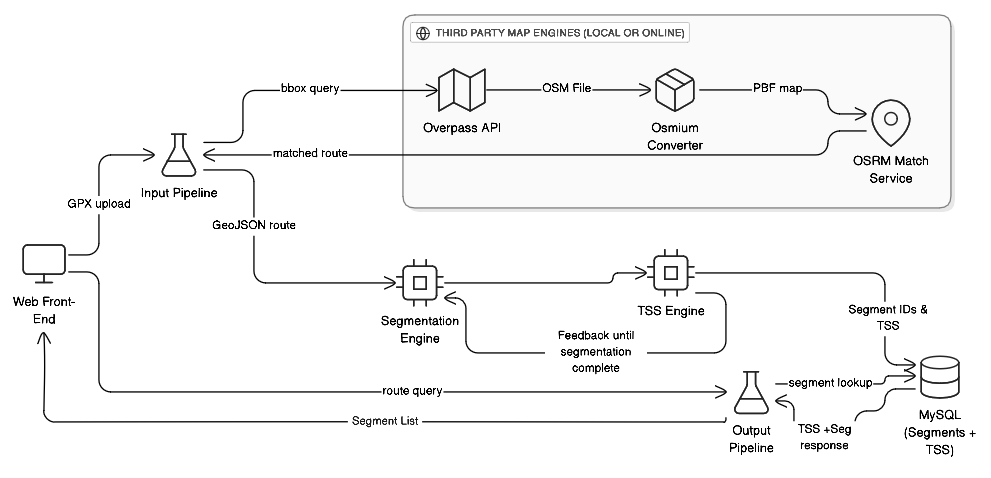
\includegraphics[width=0.9\textwidth]{archdiagram.png}
	\caption {High level system architecture for the Route Segmentation and Analysis System}
	\label{fig:archdiagram}
\end{figure}

\subsection{Architectural Views}
\subsubsection{Concept View}
The architectural concept of the system can be broken down into 3 layers:
\begin{itemize}
	\item \textbf{Presentation Layer} - This is the front end; A web application where users can either upload their GPX
	      files, or draw a route on an interactive map. This layer will communicate with the back end through HTTP API requests. This layer is mostly
	      outside the scope of the project, since I am not a front end engineer.
	\item \textbf{Processing Layer} - The beef of the project, this includes the back-end of the system, and consists of input/output pipelines,
	      and several processing engines. It will also contain several controllers, written in Python, to coordinate the pipelines and to send
	      information to and from the different engines.
	\item \textbf{Data Layer} - This layer is represented by a SQL database that stores permenant information about route segments. External APIs also
	      fall into this category, such as the Overpass API \citep{OverpassAPI} to fetch map data from online. These components provide necessary data but are mostly abstracted
	      away, in the processing layer.
\end{itemize}
\subsubsection{Functional View}
The functional view includes key modules and their responsibilities.
\begin{itemize}
	\item \textbf{Front end Web App:} Serves HTTP pages and gets information from the user.
	\item \textbf{Front End Controller:} Takes user information and routes it to correct API endpoint.
	\item \textbf{Input Pipeline Orchestrator:} Controller that handles input information routing, sending the GPX files to the pipeline, and pulling the resulting GeoJSON objects out.
	\item \textbf{Engine Orchestrator:} Takes routes, passes them to Segmentation algorithm, and handles the "two pass" system between Segmentation and TSS Engines.
	\item \textbf{DTO Orchestrator:} Formats the resulting segments, into the correct Data Object and passes it to SQL Database
	\item \textbf{Output Pipeline Orchestrator:} Receives the Route data from the Input Pipeline Orchestrator, validates it and sends it to Segmentation Engine. Gets segment list, and routes it back to front end in GeoJson format.
	\item \textbf{Segmentation Engine:} Written in C++, the engine is a specialized service that performs route segmentation and matching logic.
	\item \textbf{TSS Engine:} Takes a list of segments and the input GPX data, and assigns scores based on the training data that happens during each segment
	\item \textbf{SQL Database:} Stores all persistent segments, along with a hit count, and a list of TSS objects that have been calculated on matching segments.
	\item \textbf{Osmium Engine:} A docker service that runs a .osm to .pbf conversion and merging process. Used in the input pipeline
	\item \textbf{OSRM \citep{Luxen2011} Matching Engine:} Another docker service that takes small GeoJson chunks, and matches them to a map network.
\end{itemize}

\subsubsection{Physical View}
Hardware deployment and network design.
%TODO: Include diagrams of network design, and list of hardware items for the project
\subsubsection{Information View}
Data Flow Diagram, and Database Schema diagrams
%TODO: Implement Data flow diagram, Relational Diagrams
\subsubsection{Behavioral View}
Use case and sequence diagrams for the system
%TODO: Create and include both use case and sequence diagrams

\subsection{Design Rationale}
The choice to go with a \textbf{Pipeline Architecture} for processing data is motivated by the main use case. Users who are looking
to find a route to ride are not interested in uploading GPX, but conversely, users who are done with their ride aren't looking to
find a route. So cyclists can be considered to be in one of two states when wishing to interact with the system, either wanting a route,
or wanting to upload their data. The two pipelines reflect this with one being a GPX upload-only pipeline, and the other one is a visualisation
pipeline that shows users what their mapped route's suitibility looks like.
A simple LAMP-like stack approach is a simple, but effective pattern that can implement this project. As of right now, this is a small scale
experiment to prove the concept. If this application becomes popular, there will be several avenues to explore for scalability, such as deploying the
system to expandable cloud services such as AWS or Azure. This is beyond the scope of the project however.

\subsection{Design Patterns and Styles}
Identify and describe any applied patterns (e.g., MVC, layered) and coding conventions.
%TODO: Research and include design patterns and coding standards

\section{Module-Level Design}
\label{sec:moduledesign}
\subsection{GPX-to-Enriched-JSON Pipeline Modules}
Python Modules for the input pipeline, including dependencies, and interfaces.

\subsubsection{Module Dependency Diagram}
% \ref{fig:moddepdiag} visually shows the dependencies for each module in the input pipeline.


\subsubsection{Module Specifications}
\paragraph{gpx\_utils.py}
\begin{description}
	\small
	\item[Name:] Purpose and description.
	\item[Interfaces:] Inputs, outputs, and protocols.
	\item[Behavior:] Algorithmic overview or pseudocode.
	\item[Dependencies:] Internal and external module links.
\end{description}
\paragraph{osrm\_utils.py}
\begin{description}
	\small
	\item[Name:] Purpose and description.
	\item[Interfaces:] Inputs, outputs, and protocols.
	\item[Behavior:] Algorithmic overview or pseudocode.
	\item[Dependencies:] Internal and external module links.
\end{description}
\paragraph{osm\_utils.py}
\begin{description}
	\small
	\item[Name:] Purpose and description.
	\item[Interfaces:] Inputs, outputs, and protocols.
	\item[Behavior:] Algorithmic overview or pseudocode.
	\item[Dependencies:] Internal and external module links.
\end{description}
\paragraph{extension\_utils.py}
\begin{description}
	\small
	\item[Name:] Purpose and description.
	\item[Interfaces:] Inputs, outputs, and protocols.
	\item[Behavior:] Algorithmic overview or pseudocode.
	\item[Dependencies:] Internal and external module links.
\end{description}
\paragraph{prepare\_map.py}
\begin{description}
	\small
	\item[Name:] Purpose and description.
	\item[Interfaces:] Inputs, outputs, and protocols.
	\item[Behavior:] Algorithmic overview or pseudocode.
	\item[Dependencies:] Internal and external module links.
\end{description}
\paragraph{batch\_route\_calc.py}
\begin{description}
	\small
	\item[Name:] Purpose and description.
	\item[Interfaces:] Inputs, outputs, and protocols.
	\item[Behavior:] Algorithmic overview or pseudocode.
	\item[Dependencies:] Internal and external module links.
\end{description}
\paragraph{merge\_routes.py}
\begin{description}
	\small
	\item[Name:] Purpose and description.
	\item[Interfaces:] Inputs, outputs, and protocols.
	\item[Behavior:] Algorithmic overview or pseudocode.
	\item[Dependencies:] Internal and external module links.
\end{description}
\paragraph{build\_way\_index.py}
\begin{description}
	\small
	\item[Name:] Purpose and description.
	\item[Interfaces:] Inputs, outputs, and protocols.
	\item[Behavior:] Algorithmic overview or pseudocode.
	\item[Dependencies:] Internal and external module links.
\end{description}
\paragraph{gpx\_enrich.py}
\begin{description}
	\small
	\item[Name:] Purpose and description.
	\item[Interfaces:] Inputs, outputs, and protocols.
	\item[Behavior:] Algorithmic overview or pseudocode.
	\item[Dependencies:] Internal and external module links.
\end{description}
\paragraph{batch\_enrich.py}
\begin{description}
	\small
	\item[Name:] Purpose and description.
	\item[Interfaces:] Inputs, outputs, and protocols.
	\item[Behavior:] Algorithmic overview or pseudocode.
	\item[Dependencies:] Internal and external module links.
\end{description}

\section{Interface Design}
\subsection{User Interface}
The user interface for the project scope will just be a basic file submission system, and an interactive mapping software that can output GeoJSON
\subsection{Software Interfaces}
The front end will send GeoJSON objects to the backend via POST. GPX files can also be sent via POST with \texttt{\small Content-Type:application/gpx+xml}
The back-end will also respond with the same GeoJSON objects back to the front-end, as well as sending segment list via POST.
REST APIs are also used to interface with third party tools such as the OSRM \citep{Luxen2011} route matching engine, and the Overpass API \citep{OverpassAPI}.

\section{Data Design}
\subsection{Data Models}
ERD showing data entities and relationships.

\subsection{Database Schema}
Detailed table definitions, keys, indexes, and normalization rules.

\subsection{Data Dictionary}
Definitions and formats for all data elements used in the system.


\section{Standards and Compliance in Design}
List all applicable ISO/IEC, IEEE, and domain-specific standards adhered to (e.g., ISO/IEC 27001 \citep{ISO27001} for security).

\chapter{Methodology}
\label{chap:methodology}
% Implementation details.

\section{Component Breakdown}
This section provides a personal overview of how I went about implementing each component of the system. Rather than a dry description of what each module does (see Chapter~\ref{chap:implement} for those details), I recount the major steps I took and the rationale behind them.
\subsection{Input Pipeline}
I began by experimenting with small GPX files in order to understand the XML structure and isolate coordinate pairs. My first prototype simply read a GPX and produced a list of latitude--longitude tuples. Once I was comfortable with the data, I wrote a Python module to fetch map data from the Overpass API \citep{OverpassAPI}; this involved generating a bounding box from the GPX extents and sending the appropriate HTTP requests.

To support more complex workflows I created a Python virtual environment, installed the required dependencies from \texttt{requirements.txt} and started wrapping individual steps into scripts. After downloading raw \texttt{.osm} files I realised they needed to be converted to Protocolbuffer (\texttt{.pbf}) format for OSRM \citep{Luxen2011}, so I built a Docker image containing Osmium \citep{Osmium} and wrote a docker-compose configuration to run the conversion. Along the way I wrote helper scripts to merge multiple map tiles and orchestrated them all with a bash script called \texttt{run\_pipeline.sh}.

With the map conversion automated, I spun up OSRM in its own Docker container and tuned its \texttt{profile.lua} to better reflect cycling speeds on different surfaces. This involved a lot of trial and error: I adjusted speed values for roads, gravel and tracks, and even discovered missing road types (e.g., trunks) which required adding to the profile. After several days of tweaking I achieved reliable matching on most of my test rides.

I also developed \texttt{batch\_route\_calc.py} to handle large GPX files. This script chunks long tracks into smaller segments, submits them to OSRM in parallel using \texttt{ThreadPoolExecutor} and then merges the matched fragments. Parallelising the API requests and file operations reduced processing times from minutes to seconds. Finally I integrated visual checks with Folium \citep{folium} to verify that the matched routes and original GPX tracks aligned.

Towards the end of building the pipeline I experimented with the OSRM radius parameter and dynamic search windows to strike a balance between robust matching and avoiding spurious routes. Once the matching behaved acceptably, I moved on to enriching the matched GeoJSON with OSM metadata and GPX sensor data (described in the next subsection).

% -------------------------------------------------------
% Begin new enrichment subsection inserted here
\subsubsection{GPX Data Enrichment}\label{sec:gpx_enrich}
After I had reliable map matching in place, I turned my attention to enriching each trackpoint with context and sensor data. I wrote two Python modules, \texttt{gpx\_enrich.py} and \texttt{batch\_enrich.py}, to handle this job. These scripts take the matched GeoJSON and the original GPX files, extract the sensor readings from the \texttt{<extensions>} elements, pull out standard metadata (creator, device model, track name) and normalise all of the fields using a configuration file, \texttt{config/extensions\_map.json}. In practice I followed these steps:
\begin{enumerate}
	\item \textbf{Loading the extension rules.} I designed \texttt{extensions\_map.json} to define a set of canonical keys such as \emph{hr\_bpm}, \emph{cad\_rpm}, \emph{power\_w}, \emph{temp\_c}, \emph{speed\_mps}, \emph{alt\_m} and \emph{grade\_pct}. Each entry lists the synonyms I've encountered in GPX files (for example, ``heartrate'', ``hr'' and ``heart\_rate'' all map to \emph{hr\_bpm}) and specifies type conversions and unit transforms. When my enrichment code sees a raw GPX extension it looks up the rule, coerces the value to a number and applies any required unit conversions.
	\item \textbf{Parsing and extraction.} For each GPX file I iterate through every trackpoint, recording latitude, longitude and timestamp. I also collect any extension fields present, and attach the GPX-level metadata. This stage required careful handling of optional fields because different devices embed different sets of sensors.
	\item \textbf{Attaching OSM metadata.} Using the previously matched GeoJSON, I map each trackpoint to an OpenStreetMap way identifier via a nearest-node lookup. With this identifier I can fetch attributes like road type, name, speed limit and width from the pre-indexed OSM database described in Section~\ref{sec:wayindex}.
	\item \textbf{Producing enriched JSON.} For every point I emit an object that records its position and time, a \texttt{gpx\_list} array of canonical field objects (each with \texttt{name}, \texttt{value} and \texttt{unit}), the \texttt{way\_id}, and any associated metadata. This normalised structure became the foundation for my segmentation and training suitability scoring.
\end{enumerate}
This process gave me a clean, uniform representation of each ride, ready to be fed into the segmentation engine. Table~\ref{tab:extensionsmap} summarises some of the canonical keys and their common synonyms defined in \texttt{extensions\_map.json}. Only short phrases or keywords are included in the table to avoid overly long entries.
\begin{table}[H]
	\centering
	\caption{Canonical extension keys and example synonyms}
	\label{tab:extensionsmap}
	\begin{tabular}{ll}
		\toprule
		Canonical key       & Example GPX synonyms                                 \\
		\midrule
		\texttt{hr\_bpm}    & heartrate, heart\_rate, hr                           \\
		\texttt{cad\_rpm}   & cadence, cad\_ence, cad                              \\
		\texttt{power\_w}   & power, watts, pwr                                    \\
		\texttt{temp\_c}    & temperature, temp\_f (converted from \textdegree{}F) \\
		\texttt{speed\_mps} & speed, mph (converted to m/s), kmh                   \\
		\texttt{alt\_m}     & altitude, ele, elevation                             \\
		\texttt{grade\_pct} & grade, slope, incline                                \\
		\bottomrule
	\end{tabular}
\end{table}

\subsubsection{Pre-indexing OpenStreetMap Ways via SQLite}\label{sec:wayindex}
To efficiently map each trackpoint to its OpenStreetMap way, I build a mini database that indexes every way and its constituent edges in the downloaded map. The script \texttt{build\_way\_index.py} reads the \texttt{.pbf} map produced earlier and populates two SQLite tables:
\begin{itemize}
	\item \textbf{ways} --- one row per OSM way. Each row stores the integer \texttt{way\_id} and a JSON-encoded \texttt{tags} column containing attributes such as \texttt{highway}, \texttt{name}, \texttt{surface} and \texttt{maxspeed}. The \texttt{way\_id} column is a primary key to allow fast lookup.
	\item \textbf{edges} --- one row per directed edge between two nodes of a way. Columns store the \texttt{edge\_id} (primary key), starting node identifier \texttt{u}, ending node identifier \texttt{v}, associated \texttt{way\_id}, \texttt{direction} (1 for forward and -1 for reverse), and the geodesic length of the edge in metres. Indexes on \texttt{u} and \texttt{v} accelerate nearest-neighbour queries.
\end{itemize}
During enrichment, the coordinates of each trackpoint are snapped to the nearest OSM node using OSMnx \citep{boeing2017osmnx}. The resulting node identifier is then used to look up the corresponding \texttt{way\_id} via the \texttt{edges} table. Because the tables are indexed, this lookup is very fast even for large maps. Table~\ref{sec:wayindex} shows an example of a few rows from the \texttt{ways} and \texttt{edges} tables in our prototype database. Note that tags are abbreviated for brevity.
\begin{table}[htbp!]
	\centering
	\renewcommand{\arraystretch}{1.2} % better spacing
	\begin{tabularx}{\textwidth}{lXl}
		\toprule
		\textbf{Table}                                                     & \textbf{Columns (sample values)}                            & \textbf{Description} \\
		\midrule
		\textbf{ways}                                                      &
		(101, \{``highway'': ``residential'', ``name'': ``Main Street''\}) &
		Residential road named Main Street                                                                                                                      \\
		                                                                   & (102, \{``highway'': ``footway'', ``surface'': ``paved''\}) &
		Paved footway                                                                                                                                           \\
		\textbf{edges}                                                     &
		(1, 2, 101, 1, 50.0)                                               &
		Edge from node 1 to 2 on way 101, length 50 m                                                                                                           \\
		                                                                   & (2, 3, 101, 1, 45.0)                                        &
		Edge from node 2 to 3 on way 101, length 45 m                                                                                                           \\
		                                                                   & (3, 2, 101, -1, 45.0)                                       &
		Reverse edge from 3 back to 2 on way 101                                                                                                                \\
		\bottomrule
	\end{tabularx}
\end{table}This indexed SQLite database allows the enrichment pipeline to attach road metadata to each trackpoint in milliseconds, which is essential for scaling batch processing to thousands of GPX files.
% -------------------------------------------------------

\subsubsection{Data Stream}
The data going in was the GPX file, and the settings.yml that controlled parameters such as chunk size (of the gps chunks), and dynamic radius window, which determined how wide of a window to check for variance to adjust the match search radius.
% ...

\subsection{Segmentation Engine}

\subsubsection{Goal}
Build a C++ segmentation service that (i) runs in Docker, (ii) exposes HTTP endpoints, and (iii) processes large enriched JSON/GeoJSON (OSRM \texttt{match} output plus GPX add-ons) into a list of "segments", where each segment is
a distinct portion of the route.

\subsubsection{Step-by-step Work Log}

\begin{enumerate}
	\item \textbf{Create a minimal, conventional project layout}
	      \begin{lstlisting}[language=bash]
segmentation-engine/
├─ src/ (http/, io/, core/, models/)
├─ include/        # single-header deps: httplib, nlohmann/json
├─ config/         # settings.json
├─ scripts/        # build & run helpers
├─ CMakeLists.txt
└─ Dockerfile
    \end{lstlisting}
	      \subitem \textit{Worked:} clear separation by concern.

	\item \textbf{Initialize CMake target and fix ordering issue}
	      \begin{lstlisting}
cmake_minimum_required(VERSION 3.10)
project(segmentation_engine)
set(CMAKE_CXX_STANDARD 17)
set(CMAKE_EXPORT_COMPILE_COMMANDS ON)

add_executable(segmentation_engine
  src/main.cpp
  src/http/http_handler.cpp
  src/io/geojson_parser.cpp
  # (+ later models/ and analysis/ files)
)

target_include_directories(segmentation_engine PRIVATE include src)
target_link_libraries(segmentation_engine PRIVATE pthread)
    \end{lstlisting}
	      \subitem \textit{What failed first:} calling \texttt{target\_include\_directories} before \texttt{add\_executable}.
	      \subitem \textit{Fix:} ensure \texttt{add\_executable} precedes all \texttt{target\_*} calls.

	\item \textbf{Containerize the build (non-interactive apt)}
	      \begin{lstlisting}
FROM ubuntu:20.04
ARG DEBIAN_FRONTEND=noninteractive
ENV TZ=Etc/UTC
WORKDIR /app

RUN apt-get update && \
    apt-get install -y --no-install-recommends \
      cmake build-essential git curl && \
    rm -rf /var/lib/apt/lists/*

COPY . /app
RUN mkdir -p build && cd build && cmake .. && make -j

EXPOSE 8080
ENTRYPOINT ["/app/build/segmentation_engine"]
    \end{lstlisting}
	      \subitem \textit{Worked:} reproducible builds.
	      \subitem \textit{Earlier issue:} tzdata prompt blocking; fixed with \texttt{DEBIAN\_FRONTEND} and \texttt{TZ}.

	\item \textbf{Run script and port mapping hygiene}
	      \begin{lstlisting}[language=bash]
#!/usr/bin/env bash
set -e
IMG=segmentation_engine:latest
CTR=segmentation_container
HOST_PORT=${1:-8080}
CONTAINER_PORT=${2:-8080}

docker build -t "$IMG" .
docker rm -f "$CTR" 2>/dev/null || true
docker run -d -p "$HOST_PORT:$CONTAINER_PORT" --name "$CTR" "$IMG"
echo "http://localhost:$HOST_PORT"
    \end{lstlisting}
	      \subitem \textit{Earlier issue:} bad flag spacing caused \texttt{invalid containerPort: 5005--name}; fixed by explicit args.

	\item \textbf{Editor support (Neovim + clangd)}
	      \begin{itemize}
		      \item Enabled \texttt{CMAKE\_EXPORT\_COMPILE\_COMMANDS}.
		      \item Optional symlink: \texttt{ln -sf build/compile\_commands.json .}
		      \item clangd now sees \texttt{include/} headers.
	      \end{itemize}

	\item \textbf{HTTP server skeleton \& dispatcher}
	      \begin{lstlisting}[language=C++]
/* main.cpp: register routes by capturing `action` BY VALUE */
httplib::Server server;
server.set_payload_max_length(512ull * 1024ull * 1024ull); // large uploads
server.set_read_timeout(60,0); server.set_write_timeout(60,0);

HttpHandler handler;
server.Post("/segment", [action=std::string("segment"), &handler]
  (const auto& req, auto& res){ handler.callHandler(req,res,action); });
server.Post("/debug", [action=std::string("debug"), &handler]
  (const auto& req, auto& res){ handler.callHandler(req,res,action); });

server.listen("0.0.0.0", 8080);
    \end{lstlisting}
	      \subitem \textit{Worked:} single dispatcher \texttt{callHandler(req,res,action)}.
	      \subitem \textit{Bug caught:} capturing \texttt{action} by reference in a loop routed all paths to the last handler.

	\item \textbf{Early \texttt{/debug} tests (GeoJSON counting)}
	      \begin{itemize}
		      \item Posted a small FeatureCollection; counted \texttt{LineString}/\texttt{MultiLineString} points for a quick end-to-end proof.
	      \end{itemize}

	\item \textbf{\texttt{/debug?validate=true}: precise JSON syntax diagnostics}
	      \begin{lstlisting}[language=C++]
// On parse_error: compute byte->(line,col) and return a snippet with a caret.
auto [line, col] = calc_line_col(req.body, e.byte);
nlohmann::json err = {{"ok",false}, {"line",line}, {"column",col},
  {"context", context_snippet(req.body, e.byte)}};
res.status = 400; res.set_content(err.dump(2), "application/json");
    \end{lstlisting}
	      \subitem \textit{Worked:} fast pinpoint of malformed JSON.
	      \subitem \textit{Limitation:} does not catch type mismatches (handled next).

	\item \textbf{Accept large raw JSON bodies reliably}
	      \begin{itemize}
		      \item Increased payload limit/timeouts (see server setup above).
		      \item Confirmed \texttt{curl --data-binary @file.json} works for $\gg$15\,MB.
	      \end{itemize}

	\item \textbf{Define enriched input model (OSRM match + GPX add-ons)}
	      \begin{lstlisting}[language=C++]
// models (subset): no OSRM steps; tolerate null tracepoints; epoch times in GPX.
struct Geometry {
  std::string type; // "LineString"
  std::vector<std::array<double,2>> coordinates; // [lon,lat]
};

struct Leg {
  nlohmann::json annotation;
  std::string summary;
  double weight=0, duration=0, distance=0;
};

struct Matching {
  double confidence=0;
  Geometry geometry;
  std::vector<Leg> legs;
  std::string weight_name;
  double weight=0, duration=0, distance=0;
};

struct GpxPoint {
  double lat=0, lon=0, ele=0;
  long long time=0; // epoch seconds
  nlohmann::json extensions; // array {key,value} OR object
};

struct Tracepoint {
  bool matched=false; // supports null entries
  int alternatives_count=0, waypoint_index=-1, matchings_index=-1;
  std::array<double,2> location{0.0,0.0};
  std::string name;
  std::vector<GpxPoint> gpx_list;
};

struct OsrmMatchResponse {
  std::string code;
  std::vector<Matching>   matchings;   // rule: use first
  std::vector<Tracepoint> tracepoints; // null-safe placeholders
};
    \end{lstlisting}

	\item \textbf{Non-intrusive \texttt{from\_json} + defensive parsing}
	      \begin{lstlisting}[language=C++]
// Example: robust Geometry::from_json (no throws on null/wrong types)
inline void from_json(const nlohmann::json& j, Geometry& g) {
  if (j.contains("type") && j["type"].is_string()) g.type = j["type"].get<std::string>();
  g.coordinates.clear();
  if (j.contains("coordinates") && j["coordinates"].is_array()) {
    g.coordinates.reserve(j["coordinates"].size());
    for (const auto& pt : j["coordinates"]) {
      if (pt.is_array() && pt.size()>=2 && pt[0].is_number() && pt[1].is_number())
        g.coordinates.push_back({pt[0].get<double>(), pt[1].get<double>()});
    }
  }
}

// Tracepoint: allow null entries and keep index alignment
inline void from_json(const nlohmann::json& j, Tracepoint& t) {
  if (j.is_null()) { t.matched=false; t.waypoint_index=-1; t.matchings_index=-1; t.gpx_list.clear(); return; }
  t.matched=true;
  if (j.contains("waypoint_index") && j["waypoint_index"].is_number_integer())
    t.waypoint_index = j["waypoint_index"].get<int>();
  // ... (similar guards for other fields; parse gpx_list if array)
}
    \end{lstlisting}
	      \subitem \textit{What failed earlier:}
	      \begin{itemize}
		      \item \textbf{type\_error.302} (e.g., \texttt{"type"} was numeric somewhere): fixed by checking \texttt{is\_string()} before reading strings.
		      \item \textbf{type\_error.306} (calling \texttt{value()} on null): fixed by replacing \texttt{value()} with \texttt{contains()+is\_*()} guards.
	      \end{itemize}

	\item \textbf{Rule for multiple matchings}
	      \begin{itemize}
		      \item If \texttt{matchings.size()>0}, use \texttt{matchings.front()} and warn if more exist (consistent downstream behavior).
	      \end{itemize}

	\item \textbf{Status at this milestone}
	      \begin{itemize}
		      \item Dockerized C++ service with \texttt{/segment} and \texttt{/debug}.
		      \item Large JSON accepted and parsed into strong C++ types.
		      \item Defensive deserialization: tolerant of nulls, type variance, epoch timestamps, and extension arrays.
		      \item Ready to implement segmentation logic on the parsed model.
	      \end{itemize}
\end{enumerate}

\subsection{TSS Engine}
% ...

% Add more as needed
\section{Testing and Results}
% Testing procedures and results.

\chapter{Results and Conclusions}
\label{chap:results}
% Final results and conclusions.

\chapter{Further Discussions and Research Gaps}
\label{chap:discussion}
% Discussion and gaps.

\appendix
\chapter{Further Reading}
\label{apx:furtherreading}
\chapter{Source Code and Structures}
\label{apx:sourcecode}
\chapter{Directory Structure}
\label{apx:dirstruct}
\chapter{Application Documentation}
\label{apx:docs}

%---------------------------------------------------------------------------
% Bibliography
%---------------------------------------------------------------------------
\bibliographystyle{unsrtnat}
\bibliography{references}

\end{document}


